\chapter{Grundlagen}

Um den technischen Aufbau und die dahinterliegenden Konzepte zu verstehen und in den Zusammenhang einer Blockchain einordnen zu können, wird im folgenden Kapitel auf einige Grundlagen eingegangen, die für den weiteren Verlauf dieser Seminararbeit unabdingbar sind. Um den Rahmen dieser Seminararbeit nicht zu sprengen, wird vorausgesetzt, dass ein gewisses Grundverständnis bezüglich Hash-Funktionen und digitaler Signaturen vorhanden ist. Andernfalls kann dieses Grundverständnis in der zitierten Quelle \footnote{\parencite{Raikwar.2019}} aufgebaut werden.

% \section{Hash-Funktion}\label{sec:hash-funktion}
% Eine Hash-Funktion ist eine Funktion, die eine willkürlich lange Zeichenfolge entgegennimmt und eine Ausgabe erzeugt, die eine festgelegte Länge besitzt \footnote{\parencite[vgl.][S. 159f]{Damgard.1999}}. Ändert sich ein Zeichen des Eingabewertes, wird ein völlig unterschiedlicher Ausgabewert zurückgegeben. Dabei muss eine solche Hash-Funktion einige Eigenschaften erfüllen:

% \begin{itemize}
%     \item Kollisionsresistenz: Es muss nahezu unmöglich sein, zwei Eingabewerte $a$ und $b$ zu finden, die unter Verwendung derselben Hash-Funktion $H(x)$ den gleichen Ausgabewert $H(a) = y$ und $H(b) = y$ erzeugen \footnote{\parencite[vgl.][S. 3]{Raikwar.2019}}.
%     \item Einwegfunktion: Für einen generierten Ausgabewert $y$ muss es nahezu unmöglich sein, einen Eingabewert $a$ zu finden, der die Gleichung $H(a) = y$ erfüllt. Ferner muss es nahezu unmöglich sein, für einen gegebenen Eingabewert $a$ und einem daraus generierten Ausgabewert $y = H(a)$ einen zweiten Eingabewert $b$ zu finden, der den Ausgabewert $y = H(b)$ erzeugt \footnote{\parencite[vgl.][S. 3]{Raikwar.2019}}.
% \end{itemize}

% Solche Hash-Funktionen werden im Zusammenhang einer Blockchain dazu benutzt, um das kryptografische Rätsel beim Proof of Work von Bitcoin zu lösen, oder die privaten und öffentlichen Schlüssel der Verschlüsselung zu verwenden \footnote{\parencite[vgl.][S. 4]{Raikwar.2019}}. Wie diese Verschlüsselung genau funktioniert, wird in der nächsten Sektion erklärt.

% \section{Verschlüsselung}\label{sec:verschluesselung}
% Die Verschlüsselung, die bei einer Blockchain, beziehungsweise bei Bitcoin, zugrunde liegt ist die asymmetrische Verschlüsselung. Bei dieser Art von Verschlüsselung existieren zwei verschiedene Schlüssel: der öffentliche und der private Schlüssel \footnote{\parencite[vgl.]{entwickler.de.NaN}}. Jedoch wird diese Art von Verschlüsselung nicht verwendet, um eine Transaktion oder einen Block innerhalb der Blockchain zu verschlüsseln, sondern zu signieren \footnote{\parencite[vgl.][S. 11]{Raikwar.2019}}. Wie genau diese Signierung funktioniert, kann mit dem folgenden Bild veranschaulicht werden:

% \begin{figure}[h]
%     \begin{centering}
%         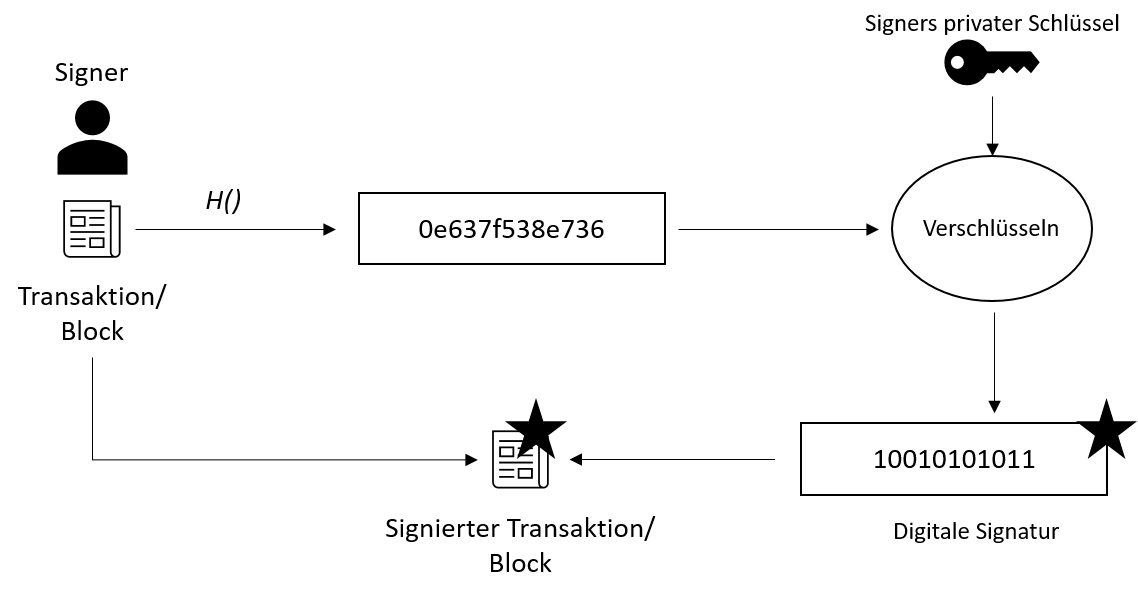
\includegraphics[width=0.7\linewidth]{Signatur_Signer.png}
%         \caption[Ablauf Signieren]{Ablauf Signieren \footnotemark}
%         \label{fig:ablauf-signieren}
%     \end{centering}
% \end{figure}
% \footnotetext{\parencite[vgl.][S. 11]{Raikwar.2019}}

% Der Ersteller (Person A) eines Blocks oder einer Transaktion generiert ein Schlüsselpaar mit einem privaten und einem öffentlichen Schlüssel. Als erstes hasht Person A seine Transaktion und verschlüsselt diese mit seinem privaten Schlüssel. Diese signiert er mit der Signatur und versendet die signierte Transaktion, die ebenfalls den öffentlichen Schlüssel beinhaltet, an das Netzwerk \footnote{\parencite[vgl.][]{entwickler.de.NaN}}

% \begin{figure}[h]
%     \begin{centering}
%         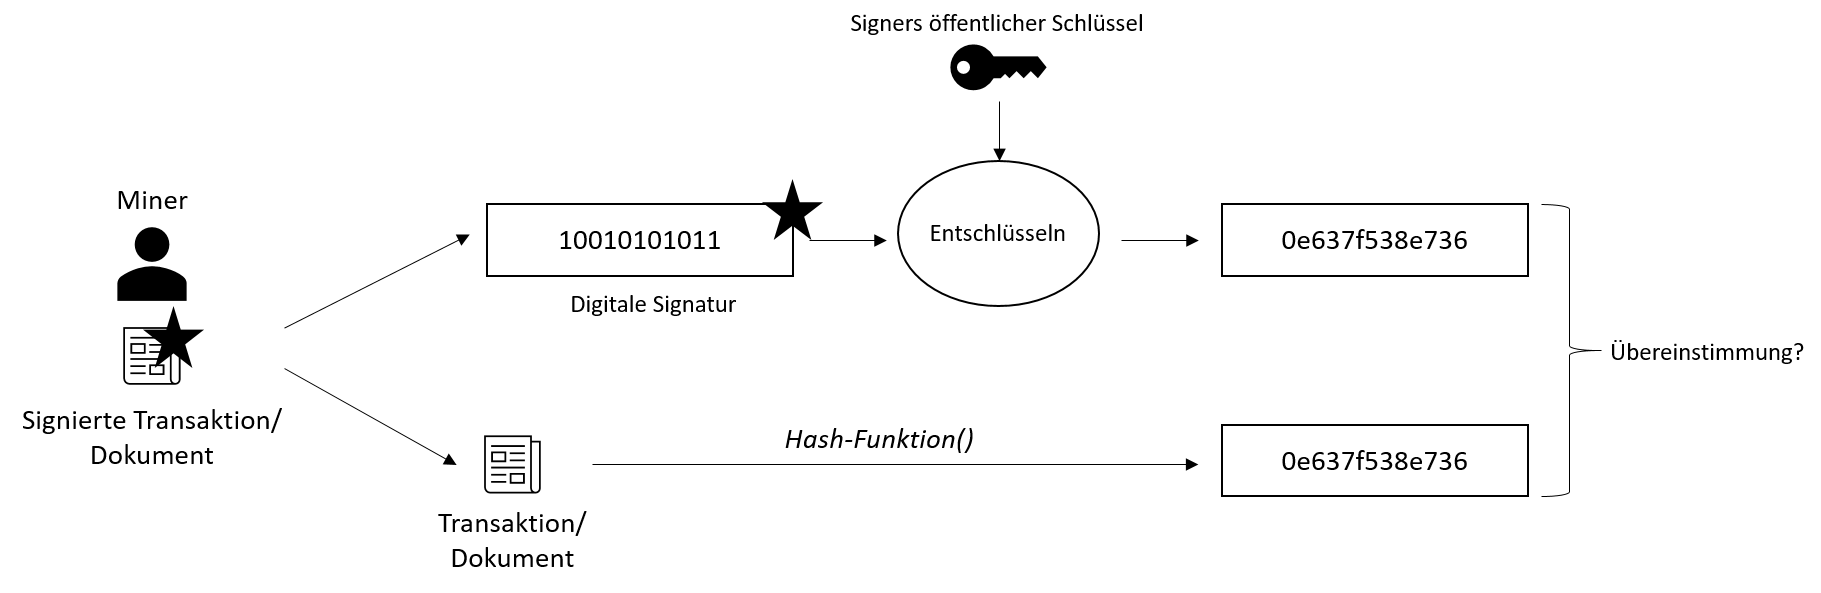
\includegraphics[width=1.0\linewidth]{Signatur_Verifier.png}
%         \caption[Ablauf Verifizieren]{Ablauf Verifizieren \footnotemark}
%         \label{fig:ablauf-verifizieren}
%     \end{centering}
% \end{figure}
% \footnotetext{\parencite[vgl.][S. 11]{Raikwar.2019}}

% Anschließend muss verifiziert werden, ob die Transaktion während des Übermittelns nicht verändert wurde. Wie bereits in \vref*{sec:hash-funktion} erklärt wurde, muss sich beispielsweise nur der Betrag der Transaktion verändern, damit der Hash nicht mehr mit dem originalen Hash übereinstimmt. Dafür entnimmt ein Verifizierer (Person B) einerseits den öffentlichen Schlüssel aus der signierten Transaktion und entschlüsselt die digitale Signatur, um somit den ursprünglichen Hash zu erhalten. Andererseits hasht Person B die Transaktion mit derselben Hash-Funktion, die bereits von Person A verwendet wurde. Gleichzeitig kann auch sichergestellt werden, dass die signierte Transaktion wirklich von Person A stammt, da die digitale Signatur ansonsten nicht mit dem privaten Schlüssel entschlüsselt werden könnte. Sind die beiden Hash-Werte identisch, ist die Transaktion valide. Falls nicht, wird diese verworfen \footnote{\parencite[vgl.][]{entwickler.de.NaN}}.





\section{Aufbau eines Blocks}\label{sec:aufbau-eines-blocks}
Die Datengrundlage einer Blockchain wird mit Blöcken gebildet, die Teil der Blockchain sind. Diese Blöcke verweisen einerseits auf den benachbarten Block der Chain und andererseits auf die Daten, die in diesem Block gespeichert werden können \footnote{\parencite[vgl.][S. 18]{Fill.2020b}}. Wie diese Daten genau gespeichert werden, wird in \vref*{sec:merkle-baum} beschrieben.
 Der Aufbau eines Blocks kann mit \vref{fig:block-aufbau} erläutert werden:

\begin{figure}[h]
    \begin{centering}
        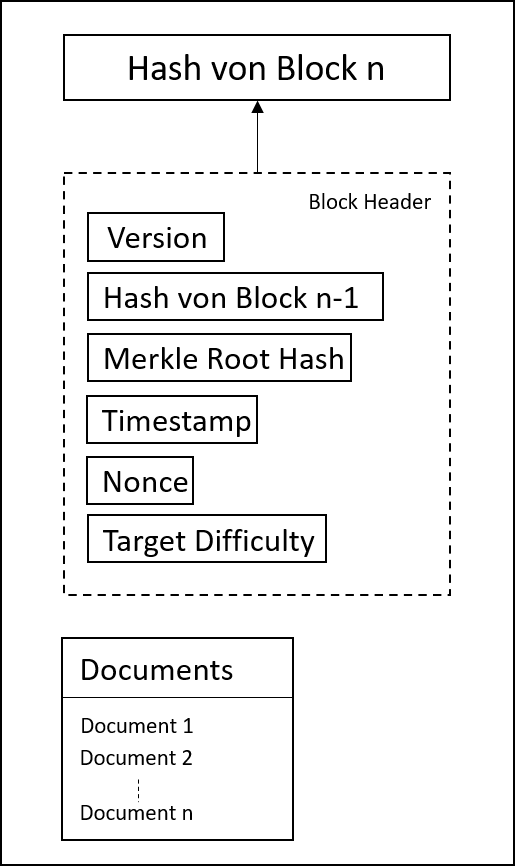
\includegraphics[width=0.4\linewidth]{Block_Aufbau.png}
        \caption[Aufbau eines Blocks]{Aufbau eines Blocks \footnotemark}
        \label{fig:block-aufbau}
    \end{centering}
\end{figure}
\footnotetext{\parencite[vgl.][S. 4]{Raikwar.2019}}

Als \textbf{Version} wird lediglich eine Version des aktuell eingesetzten Protokolls gemeint. Das Protokoll enthält Informationen über die Blockgröße, die Höhe der Belohnung eines Miners und weitere Informationen.
Damit die Blockchain als fortlaufende Kette gespeichert werden kann, muss der aktuelle Block stets auf seinen Vorgänger referenzieren. Dieser wird als Hash im Feld \textbf{Hash Block n-1} angegeben. Durch die Referenz des vorherigen Blocks entsteht eine Verkettung der einzelnen Blöcke innerhalb der Blockchain \footnote{\parencite[vgl.][S. 137]{Bruhl.2017}}. Diese Verkettung ist in \vref*{fig:blockchain-aufbau} abgebildet. Ohne die Referenz auf den vorherigen Block könnte es keine Aneinanderreihung der Blöcke geben, somit können alle fortlaufenden Blöcke aufeinander aufbauen.
In dem \textbf{Merkle-Root Hash} werden alle Transaktionen des Blocks in einem Hash gespeichert. Wie das umgesetzt wird, ist in \vref*{sec:merkle-baum} beschrieben. In der \textbf{Timestamp} wird er Zeitpunkt angegeben, bei dem der Block erstellt wird. Dieser Wert ist in Sekunden ab dem 1.1.1970 gespeichert.
In der \textbf{Difficulty} wird gespeichert, wie klein der Hash des aktuell erzeugten Blocks sein muss. Um dies zu bewerkstelligen, muss ein Hash erzeugt werden, der eine gewissen Anzahl an führenden Nullen besitzt. Je kleiner die Difficulty ist, desto schwerer ist es auch, einen Hash zu finden, der das Kriterium erfüllt. 
Da alle restlichen Komponenten des Blocks unveränderbar sind, bleibt nur noch die \textbf{Nonce} (Number only used once), um den Hash des Blocks zu beeinflussen. Sie muss von dem Miner, beschrieben in \vref*{sec:miner}, festgelegt werden, dass der erzeugte Hash den Bedingungen der Difficulty gerecht wird \footnote{\parencite[vgl.][]{Vidrih.29.12.2018}}. Wie genau der Ablauf des Minings funktioniert, wird in \vref{sec:proof-of-work} erläutert.



\section{Miner}\label{sec:miner}
Als Miner werden Teilnehmer des Blockchain-Netzwerkes bezeichnet, die Rechenleistung ihrer PCs oder anderen Geräten zur Verfügung stellen, um Daten, die in die Blockchain aufgenommen werden zu validieren - beispielsweise ob eine Person, die Bitcoins versenden will, diese auch besitzt - und diese in Blöcken zu speichern und an die bestehende Kette anzuhängen. Da für das Erstellen von neuen Blöcken Belohnungen in Form von z.B. Bitcoins vergeben werden, entsteht ein interner Wettbewerb zwischen den Minern. Dieser Wettbewer wird in \vref*{sec:proof-of-work} erläutert. Wer diesen Wettbewerb gewinnt, gewinnt auch die Belohnung.

\section{Allgemeiner Aufbau}\label{sec:allgemeiner-aufbau}
Im Allgemeinen kann eine Blockchain mit einem Datenspeicher beschrieben werden, der gleichzeitig auf mehreren Computern der am Netzwerk Teilnehmenden gespeichert ist. Die Datenstrukturen, die auf den Rechnern gespeichert werden, sind zeitlich protokolliert und somit gut nachvollziehbar und schwer veränderlich \footnote{\parencite[vgl.][]{BaFin.25.10.2021}}.
In dem verteilten Netz kann ein Teilnehmer nun nicht nur den ersten Block der Blockchain und dessen Informationen betrachten, sondern kann wie in einem digitalen Register alle Einträge durchblättern, um Daten einzusehen, die zu einem späteren Zeitpunkt in der Blockchain gespeichert wurden \footnote{\parencite[vgl.][S. 18]{Fill.2020}}.

Durch die Verteilung der Daten auf mehrere Knoten des Netzwerks hat jeder Teilnehmer die gleiche Chance, Daten zu ergänzen oder Änderungen zu dokumentieren. Analog dazu werden Änderungen für jeden Teilnehmer ersichtlich und können im Falle von Manipulationen oder korrupten Daten sofort abgewiesen werden \footnote{\parencite[vgl][]{BaFin.25.10.2021}}.

Die Tatsache, dass die Daten einer Blockchain verteilt auf das Netzwerk gespeichert sind, bringt einige Vorteile mit sich: Einerseits erhöht sich die Verfügbarkeit im Falle eines Ausfalls von einzelnen Knoten. Andererseits existiert keine zentrale Kontrollinstanz, die das Netzwerk überwacht oder Opfer eines Angriffs werden könnte \footnote{\parencite[vgl][]{BaFin.25.10.2021}}.

\begin{figure}[h]
    \begin{centering}
        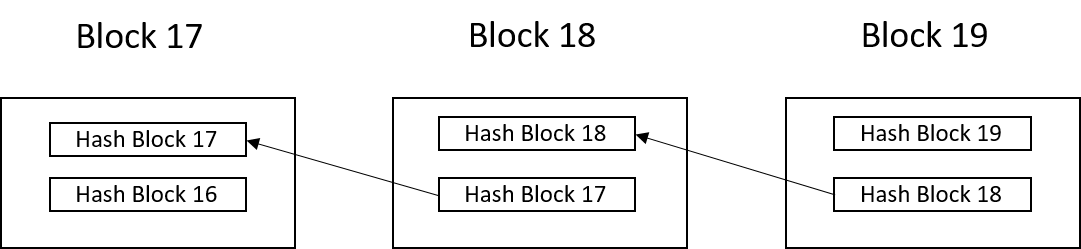
\includegraphics[width=0.8\linewidth]{Blockchain_Aufbau.png}
        \caption{Aufbau einer Blockchain}
        \label{fig:blockchain-aufbau}
    \end{centering}
\end{figure}



\section{Merkle-Baum}\label{sec:merkle-baum}
Jeder Block in einer Blockchain besteht unter anderem aus mehreren neuen Transaktionen oder Dokumenten, die in einem separaten Teil innerhalb des Blocks gespeichert werden. Alle Informationen über die Daten werden dabei nicht direkt im Header des Blocks, sondern in einen sogenannten Merkle-Hash gespeichert \footnote{\parencite[vgl.][S. 137]{Bruhl.2017}}.

Um einen solchen Hashwert zu erhalten, werden jeweils zwei benachbarte Kopien von den Daten auf der untersten Ebene des Merkle-Baums gemäß \cref{fig:Merkle-Baum} zusammengefasst und gehasht. In der nächsten Ebene werden erneut die benachbarten Hashes zu einem Hash zusammengefasst, bis sich der endgültige Merkle-Hash ergibt \footnote{\parencite[vgl.][S. 8f]{Fill.2020}}.

Anhand von einem Merkle-Hash kann überprüft werden, ob es eine noch so kleine Änderung in einem der Dokumente gegeben hat, da eine Veränderung eines Dokuments unmittelbar eine Änderung aller damit verbundenen Hashes und des Merkle-Hash mit sich zieht. Möchte nun herausgefunden werden, ob ein Dokument nachträglich verändert wurde, müssen nicht alle Dokumente auf etwaige Veränderungen analysiert werden, sondern nur deren Hashes. Werden dabei die Hashes vor und nach der Änderung der Dokumente verglichen, kann festgestellt werden, in welchem Dokument die Änderungen vorgenommen wurden. Anhand von dieser Methode kann auch festgestellt werden, ob ein bestimmtes Dokument Teil der Merkle-Baums ist \footnote{\parencite[vgl.][S. 9ff]{Fill.2020}}.


\begin{figure}[h]
    \begin{centering}
        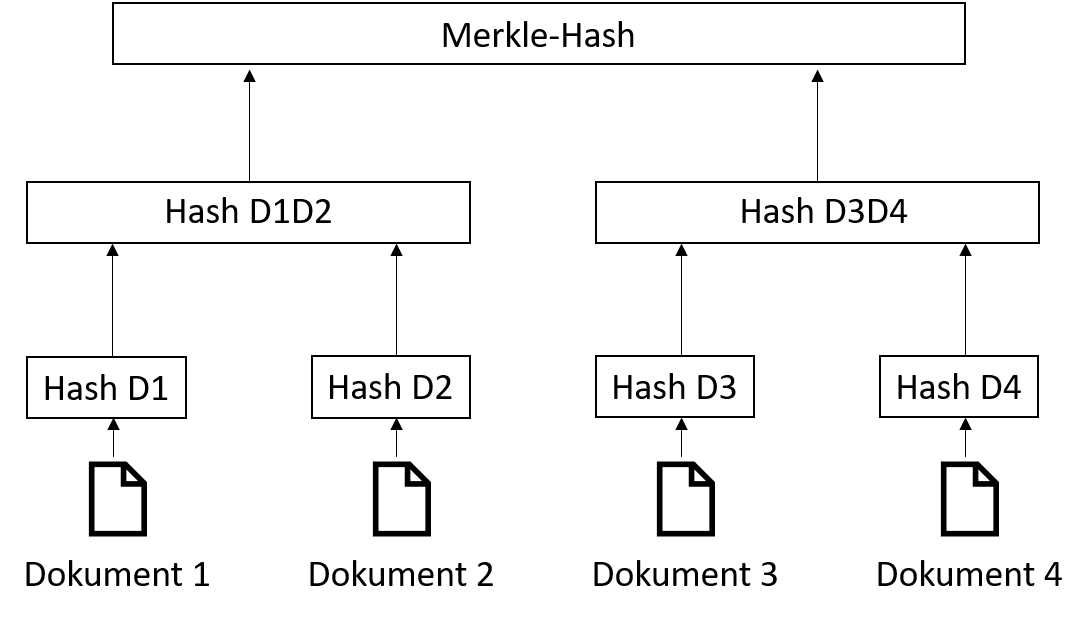
\includegraphics[width=0.8\linewidth]{Merkle-Hash.png}
        \caption[Merkle-Baum]{Merkle-Baum \footnotemark}
        \label{fig:Merkle-Baum}
    \end{centering}
\end{figure}
\footnotetext{\parencite[vgl.][S. 10]{Fill.2020}}




